%======================================================================
\subsection{MOD-05 plan: threads, holes and the hardware library (25 Oct 2026)}\label{sec:mod05-plan}
%======================================================================

\eref{MOD-05} gives Heuretes FreeCAD three things Fusion and SolidWorks users reach for every day: hole
presets (with \textbf{heat-set insert} holes for printed parts), a \textbf{cosmetic thread}, and a
\textbf{fastener library} whose screws, nuts and washers are vault COTS items. It bundles the open-source
Fasteners add-on instead of writing a library, and keeps everything else in Python next to the existing
vault engine. This chapter was written on 25 Oct and built the same evening (section~9), on your
instruction to build on my recommendations; the decisions I took are marked \emph{Decided} with the reason,
and the open ones are at the end.

\paragraph{Your decisions (25 Oct).}
\begin{center}
\small
\begin{tabularx}{\linewidth}{@{}lX@{}}
\toprule
Question & Answer\\
\midrule
Fastener library & The \textbf{Fasteners add-on} (\code{shaise/FreeCAD\_FastenersWB}: ISO/DIN screws, nuts,
  washers, inserts), bundled with Heuretes FreeCAD.\\
In the vault & A fastener placed in an assembly is a vault \textbf{COTS item} (item type \code{cots}) with a
  Heuretes FreeCAD part number.\\
Heat-set holes & \textbf{Ruthex / CNC Kitchen, M2--M5}, with their published hole diameters and depths.\\
Open details & Decided here with reasons; questions listed in section~8.\\
\bottomrule
\end{tabularx}
\end{center}

%----------------------------------------------------------------------
\subsubsection*{1. What FreeCAD 1.1 already has}

\begin{center}
\small
\begin{tabularx}{\linewidth}{@{}lX@{}}
\toprule
Where & What it does, and what it lacks\\
\midrule
PartDesign \code{Hole} & Thread type (ISO metric coarse and fine, UNC/UNF/UNEF, NPT, BSP, ...), size, class
  (6H \dots), clearance fit (Fine / Medium / Coarse, ISO~273), counterbore and countersink from tables
  (\file{Resources/Hole/iso4762.json} and nine more), drill point, thread depth (\emph{Hole depth},
  \emph{Dimension}, \emph{Tapped (DIN76)}). \code{Threaded} with \code{ModelThread} off cuts the tap drill and
  keeps the thread as data; with it on, the helix is modelled (for printing).
  \emph{Lacks:} named presets, heat-set inserts, any 3D sign that a hole is threaded.\\
TechDraw & Four extension commands (\emph{Thread Hole Side}, \emph{Hole Bottom}, \emph{Bolt Side},
  \emph{Bolt Bottom}) draw cosmetic thread lines on a view, by hand, from picked edges.
  \emph{Lacks:} callouts written from the model; nothing follows when the hole changes.\\
Fasteners & Not bundled; installed from the Addon Manager (network) by those who know it.\\
\bottomrule
\end{tabularx}
\end{center}

%----------------------------------------------------------------------
\subsubsection*{2. Hole presets and heat-set inserts}

\textbf{Decided:} a preset is a named set of values for an ordinary PartDesign \code{Hole}, not a new
feature. \emph{Reason:} the Hole already computes clearance, tap drill, counterbore and countersink from
standard tables and has a task panel; a preset only has to fill it. After the preset the Hole's own panel
edits it as usual, and the preset's name stays on the hole (property \code{HolePreset}) so the callout can
say \emph{heat-set insert}. Presets live in \file{config/hole\_presets.json} (built in) and
\file{<vault>/hole\_presets.json}: a vault preset of the same name replaces the built-in one, so a shop
that prints PETG or uses another insert tunes its numbers once, for everyone.

\paragraph{Heat-set inserts: why the numbers are what they are.} A heat-set insert is pressed in with a
soldering iron at about the plastic's melting point; its knurls melt their way in and the plastic flows
back into the knurls as it cools. The printed hole is therefore \emph{smaller} than the insert's outside
diameter $D_o$ (so there is plastic to grip) and \emph{larger} than the thread's major diameter (so the
insert starts straight). The displaced plastic has to go somewhere: per insert it is about
\[
  V \approx \tfrac{\pi}{4}\,(D_o^2 - d_h^2)\,L ,
\]
for M3 ($D_o=4.6$, $d_h=4.0$, $L=5.7$) $V\approx 23$\,mm$^3$. Most of it flows into the knurls and the
wall; the hole is made about \textbf{1\,mm deeper than the insert} so the rest gathers below it instead of
lifting the insert or closing the thread. That is both makers' advice, and the presets use
$\text{depth} = L + 1$. The wall around the insert has to carry the pull-out load; both makers give a
minimum wall of roughly $1.3$--$2$\,mm, stored with the preset (\code{min\_wall}) for a future check.

\begin{center}
\small
\begin{tabularx}{\linewidth}{@{}llrrrrX@{}}
\toprule
Preset & Thread & $L$ & $D_o$ & Hole $d_h$ & Depth & Inserts it is for\\
\midrule
Heat-set M2x3 & M2 & 3.0 & 3.6 & 3.2 & 4.0 & CNC Kitchen M2$\times$3\\
Heat-set M2x4 & M2 & 4.0 & 3.7 & 3.2 & 5.0 & ruthex RX-M2x4\\
Heat-set M2.5x4 & M2.5 & 4.0 & 4.0 & 3.6 & 5.0 & CNC Kitchen M2.5$\times$4\\
Heat-set M2.5x5.7 & M2.5 & 5.7 & 4.0 & 3.6 & 6.7 & ruthex RX-M2.5x5.7\\
Heat-set M3x4 & M3 & 4.0 & 4.6 & 4.0 & 5.0 & CNC Kitchen M3$\times$4 (short)\\
Heat-set M3x5.7 & M3 & 5.7 & 4.6 & 4.0 & 6.7 & ruthex RX-M3x5.7, CNC Kitchen M3 standard\\
Heat-set M4x8.1 & M4 & 8.1 & 6.2 & 5.6 & 9.1 & ruthex RX-M4x8.1, CNC Kitchen M4 standard\\
Heat-set M5x9.5 & M5 & 9.5 & 6.9 & 6.4 & 10.5 & ruthex RX-M5x9.5, CNC Kitchen M5 standard\\
\bottomrule
\end{tabularx}
\end{center}
\emph{Source and caveat.} The hole diameters ($3.2$, $3.6$, $4.0$, $5.6$, $6.4$\,mm for M2, M2.5, M3, M4,
M5) and the insert lengths are the values both makers publish on their product pages and data sheets, as I
know them; this session had no web access beyond the add-on download, so they could not be re-read
today; the add-on's own insert table agrees for M2, M3, M4 and M5 (section~4). Every heat-set preset therefore carries \code{"checked": false} until you (or I, with web access)
compare it with the data sheet in hand (question~1). The outside diameters $D_o$ are only used for the
theory above and the wall check, not for the hole.

\paragraph{The other presets} come straight from the Hole's tables: \emph{Tapped} M2--M6 (ISO metric coarse,
6H, thread $1.5$--$2\,d$ deep, drill point $118^\circ$, \code{ModelThread} off), \emph{Clearance} M2--M6
(ISO~273 medium, through), \emph{Counterbore} M3--M5 for ISO~4762 heads, \emph{Countersink} M3--M4 for
ISO~10642. The command is \emph{Hole Preset} (\code{BruceWorx\_HolePreset}) on the Solid tab next to Hole:
with a Hole selected it re-presets it; with a sketch, face or points selected it makes the Hole first.

%----------------------------------------------------------------------
\subsubsection*{3. The cosmetic thread object}

\textbf{Decided:} ``cosmetic thread'' means \emph{a thread recorded on a cylindrical face, shown the way a
drawing shows it, that does not change the solid.} Concretely a \code{CosmeticThread} object
(\code{Part::FeaturePython}) with a face link, designation (\code{M3}, \code{M8x1}), internal/external,
length (from either end), tolerance class, and a read-only \code{Callout}. It draws the \emph{other}
diameter, as a drawing would (a tapped hole's major diameter, a bolt's minor diameter $d_3$), as thin dashed
circles at both ends and four lines between them, drawn without the depth test so they show through the
solid the way a hidden thread does; the thread starts at the face's open end (a blind hole's entry, a
stud's free end; \code{FromOtherEnd} flips it); the designation is guessed from the face (a hole's
diameter against the tap drill and $D_1$, a shaft's against $d$). It sits beside the body in the part, so
a link to the part in an assembly shows it too.

\emph{Reasons.} PartDesign Holes already carry thread data, so they need no extra object: the callout reads
the Hole. What is missing is (a) \textbf{external} threads (studs, shafts, the threaded end of a turned part),
which no FreeCAD feature records, and (b) threads on holes that are \textbf{not} PartDesign Holes (STEP
imports, Part workbench cuts). Fusion's and SolidWorks' cosmetic threads are exactly that and are also drawn
as a texture; a texture on one face is a renderer change (another agent's area), so the dashed geometry
is the first step and the texture is question~4. With ISO~68-1: $H=\tfrac{\sqrt3}{2}P$,
$D_1=d-1.0825P$, $d_3=d-1.2269P$ (the drawn circles and
guessing the size).

%----------------------------------------------------------------------
\subsubsection*{4. Bundling the Fasteners add-on}

\begin{center}
\small
\begin{tabularx}{\linewidth}{@{}lX@{}}
\toprule
Item & Finding\\
\midrule
Version & \textbf{0.5.67} (tag \code{V0.5.67-beta}, commit \code{fddd07a}, \file{package.xml} dated 10 Sep 2025).
  It is the newest tag and \code{master} has not moved since: the add-on is mature and quiet, maintained by
  its author (Shai Seger, also SheetMetal's).\\
Licence & \textbf{GPL-2.0-or-later} (\file{LICENSE} is the GPL-2 text; \file{package.xml} and the file headers
  agree). Unlike SheetMetal it was never relicensed to the LGPL.\\
Compatible? & Yes, as for SheetMetal's eight GPL files (\S\ref{sec:mod06-plan}): LGPL-2.1-or-later FreeCAD may
  be combined with GPL-2.0-or-later Python, and the combination is then distributed under the GPL. Its main
  duty, the complete corresponding source, \eref{FND-04} already plans (source archive per release; the add-on
  ships as Python source anyway). \textbf{For FND-04:} add Fasteners to the \emph{Third-party components} of
  \file{NOTICE} (version, commit, ``GPL-2.0-or-later''), install its \file{LICENSE} as
  \file{share/doc/BruceWorx/third-party/Fasteners-LICENSE.txt}, and state in the release notes that a
  Keystone build containing it is GPL-2.0-or-later as a whole. (Engineering reading, not legal advice.)\\
Network & \textbf{None at run time.} No \code{urllib}, \code{requests}, sockets or Qt networking in any of
  its Python files; every size comes from the CSV tables in \file{FsData/} (66 files) and the geometry is
  built with Part. It needs nothing beyond FreeCAD's own modules.\\
Size & 549 files, 4.9\,MB; the code and tables are 0.9\,MB, the icons 2.6\,MB.\\
\bottomrule
\end{tabularx}
\end{center}

\paragraph{How it is shipped} (the SheetMetal pattern):
\begin{itemize}[nosep]
  \item \textbf{Vendored} in \file{package/bruceworx/vendor/fasteners/} at the tag, every file checked against
        its git blob SHA-1 from GitHub's tree listing, recorded in \file{VENDOR.txt}. Left out: the translation
        files (0.7\,MB of \file{.qm}/\file{.ts}) and the README's screencast and pictures; nothing at run time
        reads them, and the menus are English without them.
  \item \textbf{Folder name} \file{fasteners}, the name the Addon Manager installs it under. FreeCAD keys modules
        by lower-case folder name and reads the user's \file{Mod} after the built-in one, so a copy installed
        from the Addon Manager replaces ours, as for SheetMetal.
  \item \textbf{CMake.} \code{option(BUILD\_BW\_FASTENERS ... ON)} in \file{src/Mod/CMakeLists.txt}; the
        vendor folder's \file{CMakeLists.txt} copies it into \file{<build>/Mod/fasteners} (what
        \file{build/release/bin/FreeCAD} loads) and installs it to \file{Mod/fasteners}, with its
        \file{package.xml} (it names the workbench), minus the add-on's \file{tests/}.
  \item \textbf{Keystone.} \file{make-keystone.sh} installs the build with \code{cmake --install} into
        \file{Keystone.app/Contents}, so the add-on lands in \file{Contents/Mod/fasteners} with no change to the
        script; the bundle's self-check only has to list it.
  \item \textbf{Off switch.} Preferences $\rightarrow$ BruceWorx $\rightarrow$ \emph{Fasteners add-on} (default
        on; \code{FastenersAddon}) puts \code{fasteners} on FreeCAD's \code{DisabledAddons} list in
        \file{FreeCADInit.py}, next to the SheetMetal switch. With it off, Insert Fastener says why it is
        greyed out; hole presets and cosmetic threads do not need the add-on.
  \item \textbf{Cross-check of section~2.} The add-on's own heat-set insert table (\file{FsData/HeatInserts.csv},
        type \code{IUTHeatInsert}) gives the same hole diameters for M2, M3, M4 and M5 (3.23, 4.00, 5.67,
        6.43\,mm) and the same lengths (4.0, 5.74, 8.15, 9.52\,mm), and outside diameters 3.73, 4.55, 6.17,
        6.93\,mm, which the presets now use for $D_o$. It differs for \textbf{M2.5}: it uses the M3 insert's body
        (hole 4.0\,mm), where the presets use 3.6\,mm for ruthex's smaller M2.5 (question~1).
\end{itemize}

%----------------------------------------------------------------------
\subsubsection*{5. Fasteners as vault COTS items}

\textbf{Decided:} each distinct fastener (type, size, length) is \textbf{one vault item}, item type
\code{cots}, \textbf{with its own small FreeCAD file} holding the add-on's fastener object, and assemblies
\emph{link} that file. \emph{Reasons:} the vault, the BOM walker (\file{bruceworx\_bom.py}) and the section
view's ``don't cut COTS'' (\code{cots\_links}: \code{ItemType == "cots"} on the linked object) all work on
linked part files; an object living inline in the assembly file is reported as ``(in this file)'' and is not
a vault item. One file per size is also SolidWorks Toolbox's model (one part per configuration) and
matches how the Leonardo gearbox already models its screws.

\begin{center}
\begin{tikzpicture}[font=\scriptsize,>=Stealth,node distance=6mm and 9mm,
  box/.style={draw=bwdark,rounded corners=2pt,fill=codebg,inner sep=3pt,align=center,minimum height=8mm}]
  \node[box] (cmd) {\emph{Insert Fastener}\\type, size, length};
  \node[box,right=of cmd] (key) {key\\\code{ISO4762-M3x40}};
  \node[box,right=of key] (cat) {\file{<vault>/hardware.json}\\or a matching description};
  \node[box,below=of cat] (new) {new COTS item\\file with the screw, WIP 01};
  \node[box,right=of cat] (link) {\code{App::Link} in the\\active assembly};
  \draw[->] (cmd) -- (key);
  \draw[->] (key) -- (cat);
  \draw[->] (cat) -- node[above]{found} (link);
  \draw[->] (cat) -- node[right]{none} (new);
  \draw[->] (new) -| (link);
\end{tikzpicture}
\end{center}

\begin{itemize}[nosep]
  \item \textbf{Key and description.} \code{hardware.fastener\_key} gives \code{ISO4762-M3x40} (nuts and
        washers: \code{ISO4032-M3}); the description is \emph{Socket head cap screw ISO 4762 M3x40}.
  \item \textbf{Catalogue.} \file{<vault>/hardware.json} (format \code{bruceworx.hardware}) maps keys to part
        numbers. A key not in it is also looked up by \textbf{description} among the vault's items, so the
        gearbox's existing ``Socket head cap screw M3x40 (COTS)'' (LE-01-01014-001) is found and reused
        instead of numbered twice. Written atomically, sorted.
  \item \textbf{New item.} Numbered like any part (document type Part, the vault's program), checked in as
        WIP~01 with the part properties: \code{ItemType = cots}, \code{Description}, \code{Vendor} /
        \code{VendorPartNumber} empty for you to fill, material steel, mass computed. The fastener object
        keeps the add-on's own parameters, so a file can be re-opened and inspected; its type, size and length
        are read-only there (one item, one size: insert the other size instead). A length the standard's table
        does not list is typed in (ISO~4762 lists M3 only up to 30; the gearbox's M3x40 is DIN~912's) and
        becomes the add-on's custom length.
  \item \textbf{Placing.} With a circular edge selected the link is placed on it, axis along the hole; with
        nothing selected, at the origin. Joints are \eref{ASM-09} (smart fastener mating) and not this epic.
  \item \textbf{Existing COTS parts.} The gearbox's bearings, pins, screws and motor were made as item type
        \code{part}. A new journal operation \code{set\_item\_type} (part $\leftrightarrow$ cots only, any
        state but Obsolete, recorded with who and when) and the command \emph{Mark as COTS} change them;
        the file's \code{ItemType} is set on the next check-in. \emph{Note:} a Keystone built before this
        change cannot read a vault once the operation is in its journal; rebuild Keystone before using it on
        Vector.
\end{itemize}

%----------------------------------------------------------------------
\subsubsection*{6. Callouts on the drawing}

\emph{Hole Callouts} (\code{BruceWorx\_HoleCallouts}, Drawing workspace) puts a leader and a text on the
selected view for every Hole and cosmetic thread of the part it shows, written from the model:
\begin{center}
\small
\begin{tabular}{@{}ll@{}}
\toprule
Hole & Callout\\
\midrule
Tapped M3, 6 deep in an 8 deep drill & \code{M3x0.5-6H \textdownarrow6} / \code{\O2.5 \textdownarrow8}\\
Heat-set M3x5.7 & \code{\O4 \textdownarrow6.7} / \code{HEAT-SET INSERT M3x5.7}\\
Clearance M3, through, counterbored & \code{\O3.4 THRU} / \code{counterbore \O6.5 \textdownarrow3.4}\\
Four tapped holes from one feature & \code{4X M3x0.5-6H \textdownarrow6} \dots\\
\bottomrule
\end{tabular}
\end{center}
(The real text uses the ASME/ISO depth, counterbore and countersink symbols, which osifont has.) Running it
again rewrites the text and keeps where you dragged it; a hole edited away from its preset loses the
\emph{heat-set} line. Full associativity (callouts that update on recompute, attached to the hole's edge)
is \eref{DRW-04}, which builds on this.

%----------------------------------------------------------------------
\subsubsection*{7. Acceptance on the Leonardo gearbox}

On a copy of the gearbox and of the Vector vault (the real vault is not written):
\begin{enumerate}[nosep]
  \item \emph{Mark as COTS} finds the screws (LE-01-01014/15/16), the bearings 683ZZ / 688ZZ
        (LE-01-01010/11), the dowel pin and the motor by their descriptions; after it, the vault lists them as
        COTS and \code{cots\_links} on the assembly returns the 4 M3x40, 4 M3x6, 3 683ZZ, the 688ZZ, 3 pins and
        the motor.
  \item \emph{Insert Fastener} ISO~4762 M3x40 into the assembly links \textbf{LE-01-01014-001} (found by
        description, no new number); ISO~4762 M3x12 creates one new COTS item; inserting it again reuses it.
  \item A heat-set M3x5.7 hole and a tapped M3 hole on the end cap get the callouts of section~6 on a
        drawing view.
  \item The bundled add-on loads with no network and makes an ISO~4762 M3x40 whose length (40) and head
        ($d_k=5.5$, $k=3$) match the standard (\code{TestBruceWorxHardware}).
\end{enumerate}

%----------------------------------------------------------------------
\subsubsection*{8. Build order and questions}

Pieces, each tested and committed: (1) this plan; (2) \file{hardware.py} with presets, thread maths,
callout text and the catalogue, unit-tested; (3) the vendored add-on, CMake, off switch, notices; (4) Hole
Preset, Cosmetic Thread and Hole Callouts; (5) Insert Fastener, \code{set\_item\_type} and Mark as COTS; (6)
the gearbox acceptance in the GUI.

\begin{enumerate}
  \item \textbf{Heat-set numbers.} Please check the eight heat-set rows against the CNC Kitchen and ruthex
        data sheets (or let me, with web access) and say which insert you actually stock; the presets are
        \code{checked: false} until then. \emph{Recommendation:} keep both makers; most of their sizes share
        one hole.
  \item \textbf{Vendor part numbers.} Fill \code{Vendor}/\code{VendorPartNumber} (e.g.\ McMaster, Misumi,
        Bossard) per COTS item by hand, or keep a per-vault supplier table that fills them on insert?
        \emph{Recommendation:} by hand for now; a supplier table with \eref{PDM-11}.
  \item \textbf{One file per size.} Fine, or would you rather have one file per type with sizes as
        configurations (\eref{MOD-03})? \emph{Recommendation:} one file per size; it is what the vault and the
        BOM understand today.
  \item \textbf{Thread texture.} Show cosmetic threads (and threaded Holes) with a thread texture in shaded
        view, as Fusion does? It touches the display code. \emph{Recommendation:} yes, after the studio
        rendering work settles.
  \item \textbf{Fasteners' own toolbar.} Keep the add-on's 100-odd commands reachable (a \emph{Fasteners} tab
        under Design), or only Heuretes FreeCAD' \emph{Insert Fastener}? \emph{Recommendation:} only Insert
        Fastener on the ribbon; the add-on's workbench stays under ``More workbenches''.
\end{enumerate}

%----------------------------------------------------------------------
\subsubsection*{9. Built and tested (25 Oct)}

\begin{center}
\small
\begin{tabularx}{\linewidth}{@{}lX@{}}
\toprule
Piece & Where, and what the tests showed\\
\midrule
Engine & \file{addons/BruceWorx/bruceworx/hardware.py}, \file{config/hole\_presets.json}: 25 unit tests (thread
  maths, presets, callouts, keys, the gearbox's descriptions, \file{hardware.json}). Vault:
  \code{set\_item\_type} (T13 of the PDM contract, \code{PUT /items/\{pn\}/type}), new COTS items numbered as
  parts, a file's \code{ItemType} following the vault on open; the whole engine suite passes (470 tests).\\
Add-on & \file{package/bruceworx/vendor/fasteners/} (500 files, 4.5\,MB, every blob SHA-1 checked);
  \code{BUILD\_BW\_FASTENERS}; installed to \file{Mod/fasteners} with its licence (checked with the vendor
  folder's install script into a scratch prefix); the off switch leaves it unloaded
  (\emph{``Addon fasteners not loaded: switched off''}).\\
Commands & \file{src/Mod/BruceWorx/bruceworx\_hardware.py}; \code{TestBruceWorxHardware}: 19 of 19 in the GUI,
  17 headless (two need the GUI). Every built-in preset makes a valid Hole; the heat-set M3 hole is
  $\varnothing4\times6.7$ with a flat bottom (volume to $10^{-3}$\,mm$^3$); ISO~4762 M3x40 is 43\,mm long
  with a 5.5\,mm head.\\
Gearbox & On copies of Vector and the gearbox: \emph{Mark as COTS} found 7 items (3 screws, 2 bearings,
  the dowel pin, the motor); \code{cots\_links} then returns 16 links (4 M3x40, 4 M3x6, three 683ZZ, the
  688ZZ, 3 pins, the motor). Insert Fastener M3x40 reused \textbf{LE-01-01014-001} (link \emph{M3x40 5}, on
  a hole rim of the end cap, head up); M3x12 made \textbf{LE-01-01017-001} (cots, WIP~01) and the second
  M3x12 reused it; 19 COTS links after. On the end cap, a heat-set M3x5.7 and a tapped M3 hole are valid
  and their callouts (figure~\ref{fig:mod05-built}) are on the drawing beside the existing
  ``4X $\varnothing$3.4 THRU''. The carrier's output shaft takes an M8x1.25 cosmetic thread.\\
\bottomrule
\end{tabularx}
\end{center}

\begin{figure}[!htbp]
\centering
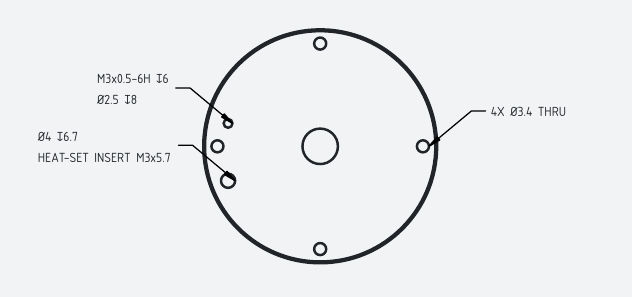
\includegraphics[width=0.52\linewidth]{fig/mod05_callouts.png}\hfill
\begin{minipage}[b]{0.44\linewidth}\centering
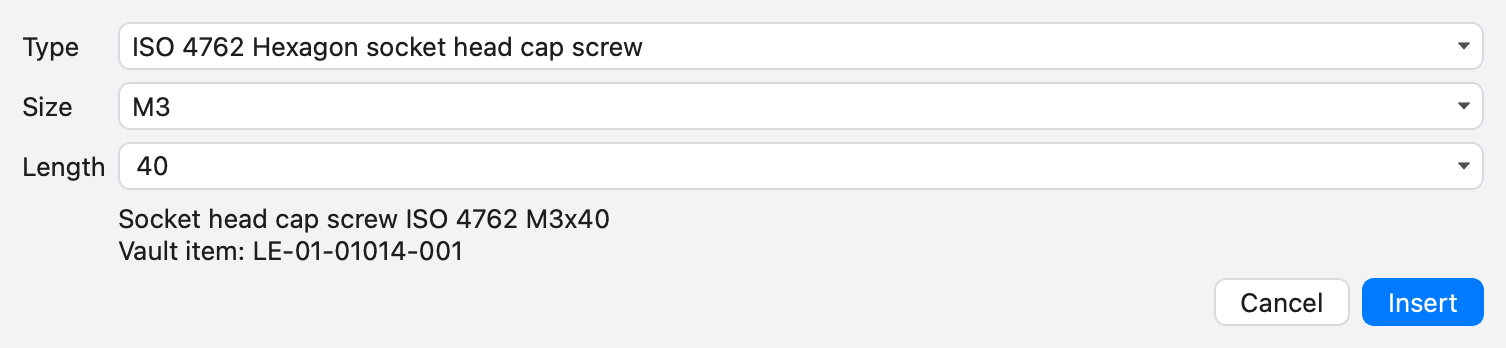
\includegraphics[width=\linewidth]{fig/mod05_insert_fastener.png}\\[6pt]
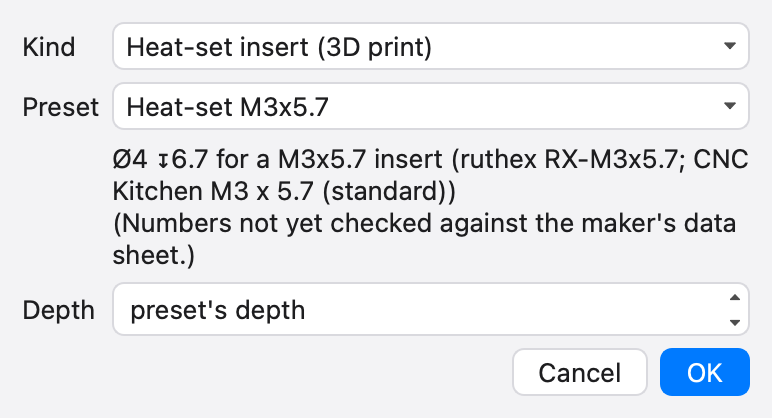
\includegraphics[width=0.75\linewidth]{fig/mod05_hole_preset.png}
\end{minipage}
\caption{Built 25 Oct. Left: the end cap's drawing with \emph{Hole Callouts}: the tapped M3 and heat-set
M3x5.7 holes added by the presets, and the part's own four clearance holes, all written from the model.
Right: \emph{Insert Fastener} with a length the standard does not list (M3x40 finds the vault's
LE-01-01014-001), and \emph{Hole Preset}.}
\label{fig:mod05-built}
\end{figure}

\paragraph{Try by hand.} Open the gearbox, select a hole rim of the end cap, \emph{Insert Fastener}
(Solid~$\rightarrow$ Assemble); in a printed part, select a sketch of circles and \emph{Hole Preset}
$\rightarrow$ Heat-set insert; on a drawing view, \emph{Hole Callouts}. Before \emph{Mark as COTS} on
Vector itself, rebuild Keystone (an older Keystone cannot read the new journal operation).
